\section{Results}\label{sec:results}
\subsection{Parameter selection and normal prediction}
The 63-fit E2 search selects ARX orders 8, 16 and 32 with ridge $10^{-7}$. Its complete normal comparison is retained in Appendix~\ref{app:earlier}. For the E5 correction, all 30 candidates produce eligible outcomes. Figure~\ref{fig:tuning} displays every development criterion, including weaker settings. Selection chooses 32 centers on all plants, width multipliers 1, 0.5 and 1, and penalties 0.01, 0.001 and 0.001 for Q1--Q3. All selected linear penalties are 0.01. These are finite normal-development choices, not parameter choices based on the attack audit.

\begin{figure*}[t]\centering
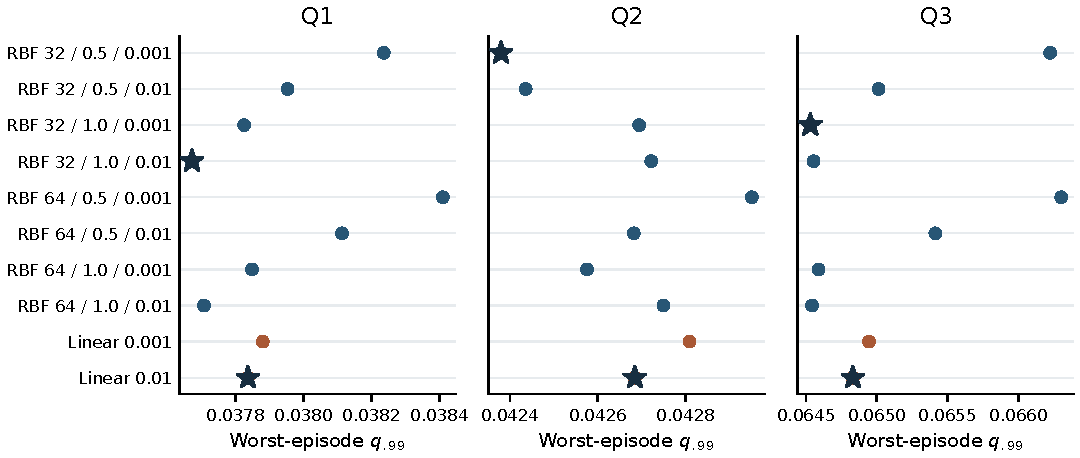
\includegraphics[width=\textwidth]{figures/tuning.pdf}
\caption{All 30 correction candidates on normal development: worst-episode 99th-percentile standardized residual (lower is better). RBF labels give centers/width multiplier/ridge; linear labels give ridge. Stars mark the selected candidate within each correction role on each plant. Horizontal scales differ across panels. These are selection outcomes, not held-out attack results.}\label{fig:tuning}
\end{figure*}

\begin{table*}[t]\centering
\caption{Selected E5 candidate and fresh-normal changes against the base reference. Positive error change is worse. Each selected RBF head has 132 coefficients, in addition to its stored centers and base model.}\label{tab:selection}
\begin{tabular}{lrrrrrrr}\toprule
Plant & ARX $p$ & Centers & Width & Ridge & $\tau$ & $\Delta$RMSE (\%) & $\Delta q_{.99}$ (\%) \\\midrule
Q1 & 8 & 32 & 1.0 & 0.01 & 0.036966 & +0.0050 & -0.1314 \\
Q2 & 16 & 32 & 0.5 & 0.001 & 0.037122 & -1.2205 & -1.4022 \\
Q3 & 32 & 32 & 1.0 & 0.001 & 0.057400 & -0.1002 & +0.1506 \\
\bottomrule\end{tabular}

\end{table*}

On 81 fresh normal episodes, RBF correction changes RMSE by +0.0050\%, $-1.2205$\% and $-0.1002$\% for Q1--Q3. Corresponding tail changes are $-0.1314$\%, $-1.4022$\% and +0.1506\%. The all-plant improvement requirement fails. Better performance on selected development episodes does not imply improvement on every new condition, and normal return-evidence availability is not post-attack clearance.

E3 tests learned prediction separately (Table~\ref{tab:imu}, Figure~\ref{fig:imu}). AR(4) achieves MSE 0.006074. All CASPER-style seeds stop at epoch 27 and select epoch 22, with MSE 0.017451--0.017703, 46.11--58.12\% below their shorter pilot errors. Compact CNN errors are 0.042700--0.044730 and still improve at epoch 100.

\begin{table*}[t]\centering
\caption{E3 normal-development prediction on the common filtered IMU prefix. Epochs are completed/selected. Every seed and deterministic control is shown; no attack metric is computed.}\label{tab:imu}
\begin{tabular}{lrrrl}\toprule
Predictor & Seed & MSE & Epochs & Stopping \\\midrule
Training mean & -- & 1.073987 & -- & Closed form \\
Persistence & -- & 0.019432 & -- & Closed form \\
AR(4) & -- & 0.006074 & -- & Closed form \\
CASPER-style CNN & 17 & 0.017703 & 27/22 & Patience \\
CASPER-style CNN & 42 & 0.017451 & 27/22 & Patience \\
CASPER-style CNN & 2026 & 0.017458 & 27/22 & Patience \\
Edge-style CNN & 17 & 0.044730 & 100/100 & Epoch limit \\
Edge-style CNN & 42 & 0.043451 & 100/100 & Epoch limit \\
Edge-style CNN & 2026 & 0.042700 & 100/100 & Epoch limit \\
\bottomrule\end{tabular}

\end{table*}
\begin{figure*}[t]\centering
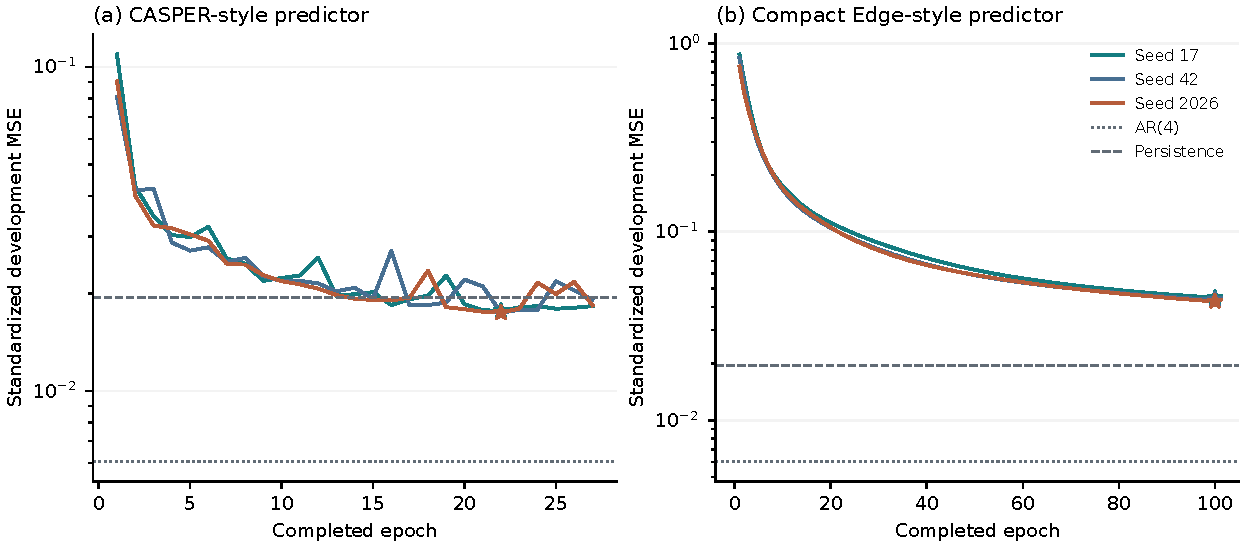
\includegraphics[width=0.85\textwidth]{figures/imu_learning_curves.pdf}
\caption{Saved E3 normal-development learning curves for all E3 neural seeds, with controls on the same targets. Patience stopping supports the adequacy of this bounded CASPER-style fit; the compact model remains limited by the epoch ceiling. These curves do not establish full-paper reproduction or attack-detection superiority.}\label{fig:imu}
\end{figure*}

Median filtering changes the prediction task and induces dependence. These normal-development errors support retaining ordinary predictors, but cannot establish attack-detection superiority or independent generalization.

\subsection{Recent author-code prediction results}
All nine recent-model runs complete on the same 2,048 normal-development targets (Table~\ref{tab:forecasts}). ModernTCN gives MSE 0.012207--0.013543; iTransformer gives MSE 0.020031--0.023680; TimeMixer gives MSE 0.011629--0.015218. All nine runs stop at their declared CPU admission limit, before the patience criterion. These values describe transferred configurations under a finite budget; they do not estimate each architecture's converged performance. Normal-development checkpoint selection also makes them unsuitable as independent test estimates. The models have 173,861, 817,153 and 58,033 parameters respectively. AR(4) remains a useful low-cost reference on these filtered targets; different histories and training budgets limit a broader architectural ranking.

\begin{table}[t]\centering
\caption{Recent author-code forecasts: all seeds, completed/selected epochs, standardized development MSE and per-seed fitting/scoring CPU. Stops: C, CPU admission; P, patience; E, epoch ceiling. No attack score is measured.}\label{tab:forecasts}
\setlength{\tabcolsep}{4pt}\begin{tabular}{llrrrl}\toprule
Model & Seed & Ep. & MSE & CPU (s) & Stop\\\midrule
ModernTCN & 17 & 4/4 & 0.013426 & 129.9 & C\\
ModernTCN & 42 & 4/4 & 0.012207 & 130.3 & C\\
ModernTCN & 2026 & 4/4 & 0.013543 & 130.4 & C\\
iTransformer & 17 & 5/4 & 0.023680 & 135.1 & C\\
iTransformer & 42 & 5/5 & 0.020875 & 135.2 & C\\
iTransformer & 2026 & 5/5 & 0.020031 & 135.1 & C\\
TimeMixer & 17 & 8/8 & 0.014041 & 130.0 & C\\
TimeMixer & 42 & 8/7 & 0.015218 & 129.9 & C\\
TimeMixer & 2026 & 8/7 & 0.011629 & 141.7 & C\\
\bottomrule\end{tabular}

\end{table}

\subsection{Five-fold temporal validation}
All 15 plant--fold fits complete, giving 4,500 scored observations per method with no failures. Table~\ref{tab:fivefold} reports every fold, pooling equal-sized plant populations after each fold's training-only standardization. The correction improves pooled error in folds four and five and in 5/15 plant--fold pairs. Its benefit is small and inconsistent. The first fold uses only 200 training observations per episode; trajectory segment and fitted scale also change across folds, so the reduction in later-fold error cannot be attributed to training size alone. This diagnostic leaves the original fit selection and attack-audit outcome unchanged.

\begin{table}[t]\centering
\caption{Five-fold chronological normal validation. Lower standardized RMSE is better. Every fold uses 900 targets; the folds reuse overlapping training prefixes.}\label{tab:fivefold}
\setlength{\tabcolsep}{4pt}\begin{tabular}{rrrr}\toprule
Fold & Targets & ARX RMSE & ARX--RBF RMSE\\\midrule
1 & 900 & 0.224181 & 0.224551\\
2 & 900 & 0.011501 & 0.011521\\
3 & 900 & 0.012052 & 0.012075\\
4 & 900 & 0.011103 & 0.011086\\
5 & 900 & 0.010940 & 0.010937\\
\bottomrule
\end{tabular}

\end{table}

\subsection{Detection and false-alarm trade-offs}
Table~\ref{tab:audit} reports the complete frozen audit. RBF dual reduces benign alarm points from 7,156 to 7,012, a 2.0123\% reduction below the required 10\%. Q1 deteriorates from 2,397 to 2,522 points, and pooled pre-return gaps increase from two to three. The primary criterion therefore fails. Base and RBF dual overlap all 108 attacks; fresh hits increase from 101 to 105. This secondary gain cannot reverse the declared failure.

\begin{table*}[t]\centering\setlength{\tabcolsep}{4pt}
\caption{All 17 registered E5 methods on 189 synthetic episodes. Benign uses 89,100 points. Hit/fresh means overlap/fresh-onset events out of 108; early is the registered continuity-based count. Clear is timely clears/detected events with return. AP evaluates continuous entry scores, not retained alarm state.}\label{tab:audit}
\begin{tabular}{lrrrrrrr}\toprule
Method & F1 & AP & Benign & Hit/fresh & Early & Gaps & Clear \\\midrule
base point & 0.7809 & 0.7276 & 853 & 108/108 & 14 & 38 & 108/108 \\
base return & 0.6452 & 0.7276 & 6,811 & 108/101 & 1 & 2 & 108/108 \\
base long & 0.6381 & 0.7276 & 7,156 & 108/101 & 1 & 2 & 108/108 \\
base dual & 0.6381 & 0.7276 & 7,156 & 108/101 & 1 & 2 & 108/108 \\
linear point & 0.7799 & 0.7276 & 895 & 108/108 & 14 & 38 & 108/108 \\
linear dual & 0.6336 & 0.7276 & 7,498 & 108/101 & 1 & 2 & 108/108 \\
RBF point & 0.7816 & 0.7276 & 835 & 108/108 & 14 & 39 & 108/108 \\
RBF return & 0.6482 & 0.7276 & 6,652 & 108/105 & 1 & 3 & 108/108 \\
RBF long & 0.6407 & 0.7276 & 7,012 & 108/105 & 1 & 3 & 108/108 \\
RBF dual & 0.6407 & 0.7276 & 7,012 & 108/105 & 1 & 3 & 108/108 \\
RBF dual, no dwell & 0.7644 & 0.7276 & 1,195 & 108/108 & 1 & 1 & 108/108 \\
following point & 0.9202 & 0.9501 & 867 & 108/108 & 108 & 6,692 & 108/108 \\
following dual & 0.7070 & 0.9501 & 7,635 & 108/105 & 90 & 2,970 & 108/108 \\
RBF following dual & 0.7069 & 0.9501 & 7,678 & 108/105 & 90 & 2,979 & 108/108 \\
persistence & 0.0333 & 0.1016 & 527 & 67/67 & 67 & 15,742 & 67/67 \\
mean (21) & 0.0082 & 0.0867 & 84 & 48/48 & 48 & 11,545 & 48/48 \\
base CUSUM & 0.4198 & 0.1967 & 857 & 108/108 & 0 & 0 & 0/108 \\
\bottomrule\end{tabular}

\end{table*}

Figure~\ref{fig:tradeoff} places schedule F1, benign occupancy and lost pre-return support beside one another. Following point has F1 0.9202 and AP 0.9501, exceeding RBF dual's 0.6407 and 0.7276. Yet it has an early falling edge on every attack, with 6,692 pre-return gap points. Following dual reduces these to 90 events and 2,970 points; base dual has one registered early-clear event and two gap points. CUSUM retains support but has no timely clearance. No single plotted axis establishes overall superiority.

\begin{figure*}[t]\centering
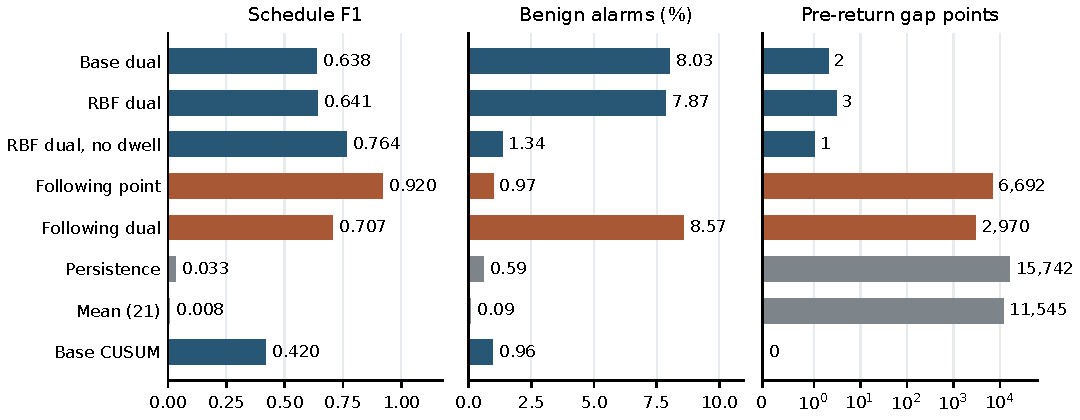
\includegraphics[width=\textwidth]{figures/tradeoffs.pdf}
\caption{Selected contrasts from the complete E5 roster: corruption-schedule F1, benign alarm occupancy and lost alarm support before physical return. Bar labels give saved values; gap axes use a logarithmic scale with a linear region near zero. The figure is a descriptive presentation of the frozen outcomes, not a newly selected primary comparison.}\label{fig:tradeoff}
\end{figure*}

\subsection{Physical return and event interpretation}
Figure~\ref{fig:trace} illustrates the distinction: schedule labels end with command corruption, while displaced motion can continue. Retaining alarm then supports recovery monitoring while reducing schedule precision.

\begin{figure*}[t]\centering
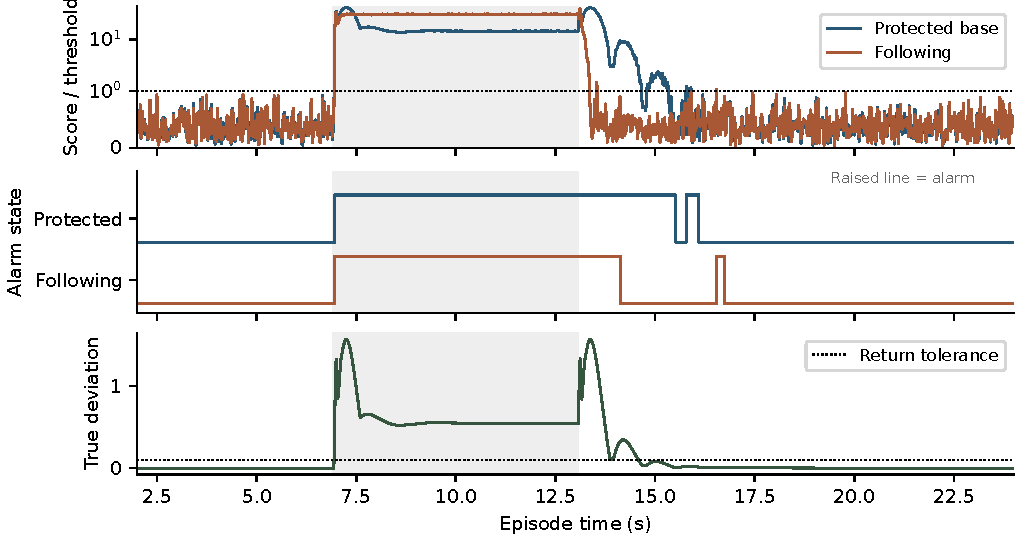
\includegraphics[width=0.77\textwidth]{figures/trace.pdf}
\caption{Post-study illustration from task N14, plant Q2, seed 17, persistent offset. Shading marks command corruption. The following residual falls while physical deviation remains above tolerance. This trace was selected to explain the aggregate contrast; it is not independent confirmatory evidence.}\label{fig:trace}
\end{figure*}

The single RBF early-clear event occurs two samples after onset, with true standardized deviation 0.01649 below tolerance 0.1. A fresh alarm starts three samples later. It is a continuity break, not an outside-tolerance clearance. A separately labelled post-study falling-edge diagnostic finds no outside-tolerance early falls for protected-reference variants, versus 108 events for following point and 82 for following dual. This clarification preserves the registered metric and failed primary decision. Persistence misses 41 events and the rolling mean misses 60; their conditional clearance fractions cannot be presented as recovery success on every event.

\subsection{Ablation and uncertainty studies}
Removing the short window changes zero alarm entries in all 189 episodes. Its contribution is unsupported under these conditions. Removing dwell reduces RBF benign points from 7,012 to 1,195, with 108 overlap hits and 108 timely clears. Its registered early-clear count remains one, on a different episode. Figure~\ref{fig:ablation} separates the component effects. The favorable no-dwell result is an exposed secondary finding; promoting it as a new confirmed detector would require a separately frozen study.

\begin{figure*}[t]\centering
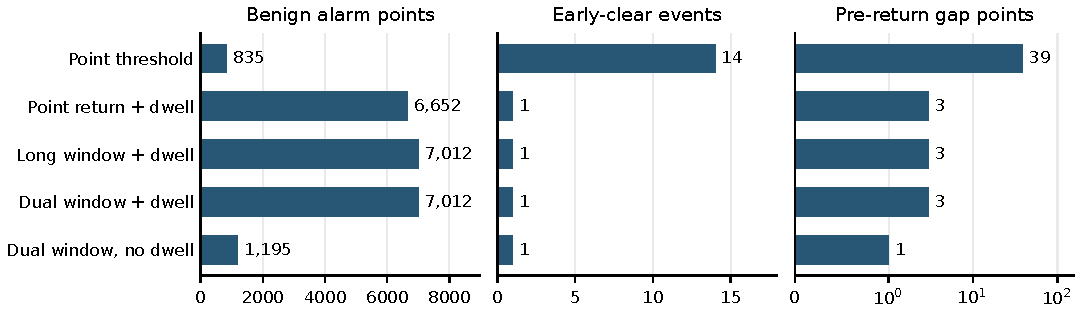
\includegraphics[width=\textwidth]{figures/ablations.pdf}
\caption{Matched RBF alarm-rule variants in E5. Entry score and calibration threshold are shared. The 41-point and dual windows produce identical alarm arrays. Dwell substantially changes benign occupancy; a small gap count alone does not account for missed events or late clearing. All variants detect and timely clear 108 events in this campaign.}\label{fig:ablation}
\end{figure*}

E1 reduces benign points from 621 to 309 using an empirical allowance, but clears only 36/108 detected events with return; its same-entry no-allowance control has 140 benign points and 108 clears. E2 reduces the harder plants' allowances by 51.27\% and 38.56\%, yet fails overall feasibility. Appendix~\ref{app:earlier} retains every earlier comparison under its distinct calibration.

E4 certifies enough normal endpoints on 20/36 constructed traces, failing its all-traces criterion. Averaging competes with temporal correlation and within-window motion. Appendix~\ref{app:uncertainty} gives the complete settings, derivation and outcomes; these are direct synthetic residuals, not attack trials.

\subsection{Computational cost and verification}
E5 normal development takes 16.115 seconds wall and 15.189 seconds worker CPU, with 53.23 MiB sampled peak memory. The final audit takes 27.515 seconds wall and 26.656 seconds CPU, with 90.17 MiB sampled memory and 83.44 MiB outputs. The IMU study takes 764.794 seconds wall, 753.252 seconds CPU and 553.05 MiB sampled memory. These are whole-pipeline measurements with shared work, not isolated inference latency or real-time guarantees.

The recent forecast campaign consumes 1208.167 seconds wall and 1199.209 seconds summed worker CPU, with 521.44 MiB maximum sampled memory and 14.48 MiB monitored outputs. All nine saved checkpoints reproduce their predictions exactly; 294 artifact and replay checks pass. The separate five-fold diagnostic uses 0.485 seconds wall and 0.297 seconds CPU and passes 109 saved-artifact checks. These are pipeline costs, not isolated inference latency.

The final audit passes 25 synthetic software tests and 30,448 saved-artifact checks, including inference replay and separate metric arithmetic. All 3,213 method--episode outcomes remain recorded. These checks support consistency with the declared implementation; they are not independent scientific replication. Appendix~\ref{app:provenance} records budgets, earlier costs and preserved failures.
